% WSCG sample document 
%
% based on Gabriel Zachmann's sample
% http://zach.in.tu-clausthal.de/latex/
%
% modified Apr 2012 to match WSCG Word template
%
\documentclass[twoside,twocolumn,10pt]{article}
%\documentclass[twoside,twocolumn,draft]{article}

%  for debugging
%\tracingall%\tracingonline=0
%\tracingparagraphs
%\tracingpages

\usepackage{biblatex}
\addbibresource{references.bib}




%%%%%%%%%%%%%%%%%%%%%%%%%%%%%%%%%%%%%%%%%%%%%%%%%%%%%%%%%%%%%%%%%%%%%%%%%%%%%
%                             Packages

\usepackage{wscg}           % includes a number of other packages (e.g., myalgorithm)
\RequirePackage{ifpdf}
\ifpdf
 \RequirePackage[pdftex]{graphicx}
 \RequirePackage[pdftex]{color}
\else
 \RequirePackage[dvips,draft]{graphicx}
 \RequirePackage[dvips]{color}
\fi
%\usepackage[german,english]{babel}     % default = english
%\usepackage{mypicture}      % loads graphicx.sty, color.sty, eepic.sty
%\usepackage{array}          % better tabular's & arrays, plus math tabular's
%\usepackage{tabularx}      % for selfadjusting p-columns
%\setlength{\extrarowheight}{1ex}   % additional space between rows
%\usepackage{booktabs}      % typographically much better
%\usepackage{mdwlist}        % for compacted lists, and more versatile lists
%\usepackage[intlimits]{amsmath} % more math stuff, see texdoc amsldoc
%\usepackage{mymath}         % own commands, loads amssymb & array.sty
%\usepackage{hyphenat}      % hyphenatable -, /, etc.
%\usepackage{theorem}
%\usepackage[sort&compress]{natbib}% better \cite commands, more flexible
%\usepackage[sort&compress,super]{natbib} % better \cite commands, more flexible
%\newcommand{\citenumfont}[1]{\textit{#1}}


\usepackage{nopageno}       % no page numbers at all; uncomment for final version
\usepackage{bm} 



%%%%%%%%%%%%%%%%%%%%%%%%%%%%%%%%%%%%%%%%%%%%%%%%%%%%%%%%%%%%%%%%%%%%%%%%%%%%%
%                                Title

\title{Simple and fast glyph rendering scheme for HARDI DWI acquisitions}

\author{
\parbox{0.25\textwidth}{\centering
Daniel Xavier Silva\\[1mm]
author's affiliation\\
1st line of address\\
2nd line of address\\
Country (ZIP) code, City, State\\[1mm]
danielxs@dca.fee.unicamp.br
}
\hspace{0.05\textwidth}
\parbox{0.25\textwidth}{\centering
Second Author\\[1mm]
author's affiliation\\
1st line of address\\
2nd line of address\\
Country (ZIP) code, City, State\\[1mm]
e@mail
}
\hspace{0.05\textwidth}
\parbox{0.25\textwidth}{\centering
Third Author\\[1mm]
author's affiliation\\
1st line of address\\
2nd line of address\\
Country (ZIP) code, City, State\\[1mm]
e@mail
}
}

%%%%%%%%%%%%%%%%%%%%%%%%%%%%%%%%%%%%%%%%%%%%%%%%%%%%%%%%%%%%%%%%%%%%%%%%%%%%%
%                          Hyperref


% no hyperlinks
\usepackage{url}
\urlstyle{tt}

% Donald Arsenau's fix for missing kerning of "//" and ":/"
\makeatletter
\def\Uslash{\mathbin{\mathchar`\/}\@ifnextchar{/}{\kern-.15em}{}}
\g@addto@macro\UrlSpecials{\do \/ {\Uslash}}
\def\Ucolon{\mathbin{\mathchar`:}\@ifnextchar{/}{\kern-.1em}{}}
\g@addto@macro\UrlSpecials{\do : {\Ucolon}}
\makeatother





%%%%%%%%%%%%%%%%%%%%%%%%%%%%%%%%%%%%%%%%%%%%%%%%%%%%%%%%%%%%%%%%%%%%%%%%%%%%%
%                              My Commands


%\DeclareMathOperator{\sgn}{sgn}

%\theorembodyfont{\upshape}
%\theoremstyle{break}
%\theoremheaderfont{\bfseries\normalsize}

%\newtheorem{lem}{Lemma}
%\newtheorem{defn}{Definition}



%%%%%%%%%%%%%%%%%%%%%%%%%%%%%%%%%%%%%%%%%%%%%%%%%%%%%%%%%%%%%%%%%%%%%%%%%%%%%
%                                Document


\begin{document}

\twocolumn[{\csname @twocolumnfalse\endcsname

\maketitle  % full width title


\begin{abstract}
\noindent



%We describe the formatting guidelines for the Journal of WSCG and WSCG proceedings adapted from the ACM and SIGGRAPH proceedings and recent WSCG templates.  Please, try to fix format of your contribution as close as possible if you use other tools.

\end{abstract}

\subsection*{Keywords}
%Keywords are your own designated keywords - Times New Roman, 10pts.
medical visualization, HARDI, computer graphics, visualization. 

\vspace*{1.0\baselineskip}
}]



%%%%%%%%%%%%%%%%%%%%%%%%%%%%%%%%%%%%%%%%%%%%%%%%%%%%%%%%%%%%%%%%%%%%%%%%%%%%%


\section{Introduction}

\copyrightspace

Diffusion weighted magnetic resonance imaging (DW-MRI) is a technique that aims to measure the random Brownian motion of water molecules. Applied to the brain, it is unique on providing in-vivo information on white matter path. Imaging methods to synthesize the diffusion signals into functions have been a subject of research more than two decades.

The first and the most used on clinic is the diffusion tensor imaging (DTI) \cite{Basser1994}, which aims to fit a set of diffusion coefficients samples into a gaussian 3D model, of average zero and the covariance matrix set by the diffusion tensor.

The limitations of DTI are well known \cite{descoteaux2015,SCHILLING2019194}. The gaussian assumption fits well the diffusion behavior when the point represents a region of the brain that one fiber passes through it, but the model is limited when it comes to describe the diffusion in points that have fibers with a more complex behavior (ie. fiber crossing, branching, kissing). This limitation affects critically the accuracy on inferring the fiber distribution in the brain.

To overcome the limitation of the gaussian model assumption, more advanced imaging methods for diffusion were introduced. These methods required more samples on the DWI than the acquisitions used on DTI and these acquisitions were labeled as High Angular Resolution Diffusion Imaging (HARDI). While the acquisitions used on DTI vary between 6 and 32, HARDI acquisitions have more than 45 \cite{descoteaux2015}.

These more advanced methods that requires a HARDI acquisition, which will be called in this work as HARDI methods, aims to reconstruct an orientation distribution function that represents the diffusion process. Some of them are model-free, which estimates the diffusion displacement from the Fourier relation between the MRI signal to its respective diffusion displacement \cite{wedeen2005, TuchQBall2004, yeh2010} and others are model-based, where they model the underlying fiber signal obtained by its respective decay on the diffusion acquisition \cite{tournier2007, tournier2007}.

The most common way to represent HARDI methods is the spherical polar plot, where a normalized version of an ODF deforms a sphere accordingly to the equation \ref{eq::normglifo}. 

\begin{equation}
\label{eq::normglifo}
    R(\bm{u}) = \frac{\psi(\bm{u}) - min(\psi(\bm{u}))}{max(\psi(\bm{u})) - min(\psi(\bm{u}))}
\end{equation}

where $\bm{u}$ is an unity vector contained in the spherical domain.

These glyphs gives a clear visualization of local information in diffusion imaging methods. It is used by researchers to attest the validity of an imaging method, the adequability of it given an acquisition and the check the relationship between the imaging method used with an algorithm of fiber reconstruction (tractography).

The color scheme used in the glyph is a function of the direction from the center of the glyph to its surface, defined in the equation \ref{eq::glyph_color}. The red color represents the mediolateral direction, green refers to the antero-posterior direction and the blue, inferior-superior direction. This color scheme is commonly used by the DWI community.


\begin{equation}
\label{eq::glyph_color}
    (r,g,b) = (|u_x|,|u_y|,|u_z|)
\end{equation}

In this work, we present a rendering scheme that aims to, given samples of ODFs associated with a spherical mesh, we render a set of spherical polar plot. The gains of performance are given by decreasing the amount of data traffic CPU-GPU by taking out redundant information on each drawing request. This is achieved by using instance rendering.

The integration of this rendering scheme in a DW-MRI visualization can be a powerful tool to the researchers in the area. It improves the understanding of the output result of an diffusion imaging method applied to DW-MRI, as well as provide an a visual information of the underlying model where directional information of fibers is extracted to be used on brain fiber reconstruction. The real time factor can improve the visual interactivity of the research in the area.


%We ask authors to follow this guideline and make paper look exactly like as this document. The easiest way to do this is simply to download a template from \cite{jou01a} and replace the content with your own.

%\section{Background}










\section{Related work}

The works in the area that have been proposed by !!ref, proposed a raycasting method.......

Up to our knowledge, there is no work in the area that uses polygons based approach to render spherical polar plots.


\section{Rendering scheme}

The approach used for rendering consists of instantiating a spherical mesh of N vertices centered on the origin and unit radius, which is sent to the GPU only once and with no repetition of vertices in the data. At each instance, the mesh is transformed by a translation matrix and its ODF samples.

The translation matrix positions the center of the spherical mesh to its respective position. The ODF samples represent the diffusion profile that are particular to each glyph. These which determines the shape of the glyph by multiplying the vertex of the mesh associated with the direction of diffusion to its ODF value.


These elements are sent from the CPU to the GPU in each drawing request that has a list of translation matrices and ODF samples as input. So, in order to achieve the goal of interactivity, it is desirable that the data traffic between both parts is as little as possible.

The traffic CPU-GPU that refers to the translation consists of sending a vector containing P translation matrices as an attribute, which is unique for each spherical mesh instantiated.

The ODF data sent to GPU consists of the N samples referring to the diffusion profiles for each of the P glyphs to be drawn. The approach used to set the ODF data and send to the GPU is by constructing a $\bm{\Psi}_{PxN}$ matrix, where P is the number of glyphs to be drawn and N is the number of samples of ODF used. The $\bm{\Psi}$ matrix is sent to the GPU as a 2D texture.


In the $\bm{\Psi}$ matrix, the element of the i-th row in the j-th column of the matrix refers to the ODF of the i-th glyph to be drawn associated with the j-th vertex of the sphere, which in turn has the coordinates of the direction $ \bm{u}_j $. We will call ODF on the i-th line of $ \psi_i(\bm{u})$ and its value at the j-th vertex of the $\psi_i(\bm{u}_j)$ sphere.

The access in the GPU of ODFs to deform its respective sphere point is done by accessing the texture data through its instance and vertex indexes in the vertex shader. To achieve this, it is necessary that the vertex index (gl\_VertexID\footnotemark) of the direction of each vertex correspond to the column of its respective ODF value $ \psi (\bm{u}_j) $ in diffusion profile matrix. The access of the rows of the diffusion profile matrix, corresponding to the diffusion profiles in its respective point is accessible by the instance index (gl\_InstanceID\footnotemark [\value{footnote}]). Having the data organized in this established way, the access is done in the using the function texelFetch\footnotemark[\value{footnote}] with the row and column access arguments through the pair ( gl\_VertexID, gl\_InstanceID)\footnotemark [\value{footnote}] \footnotetext{All commands refer to OpenGL API and GLSL shading language.}. How to access the GPU of the profile matrix is illustrated in the Fig.\ref{fig::GPU2glyph}.

\begin{figure}[htb]
    \centering
    %\rule{6cm}{3cm}
    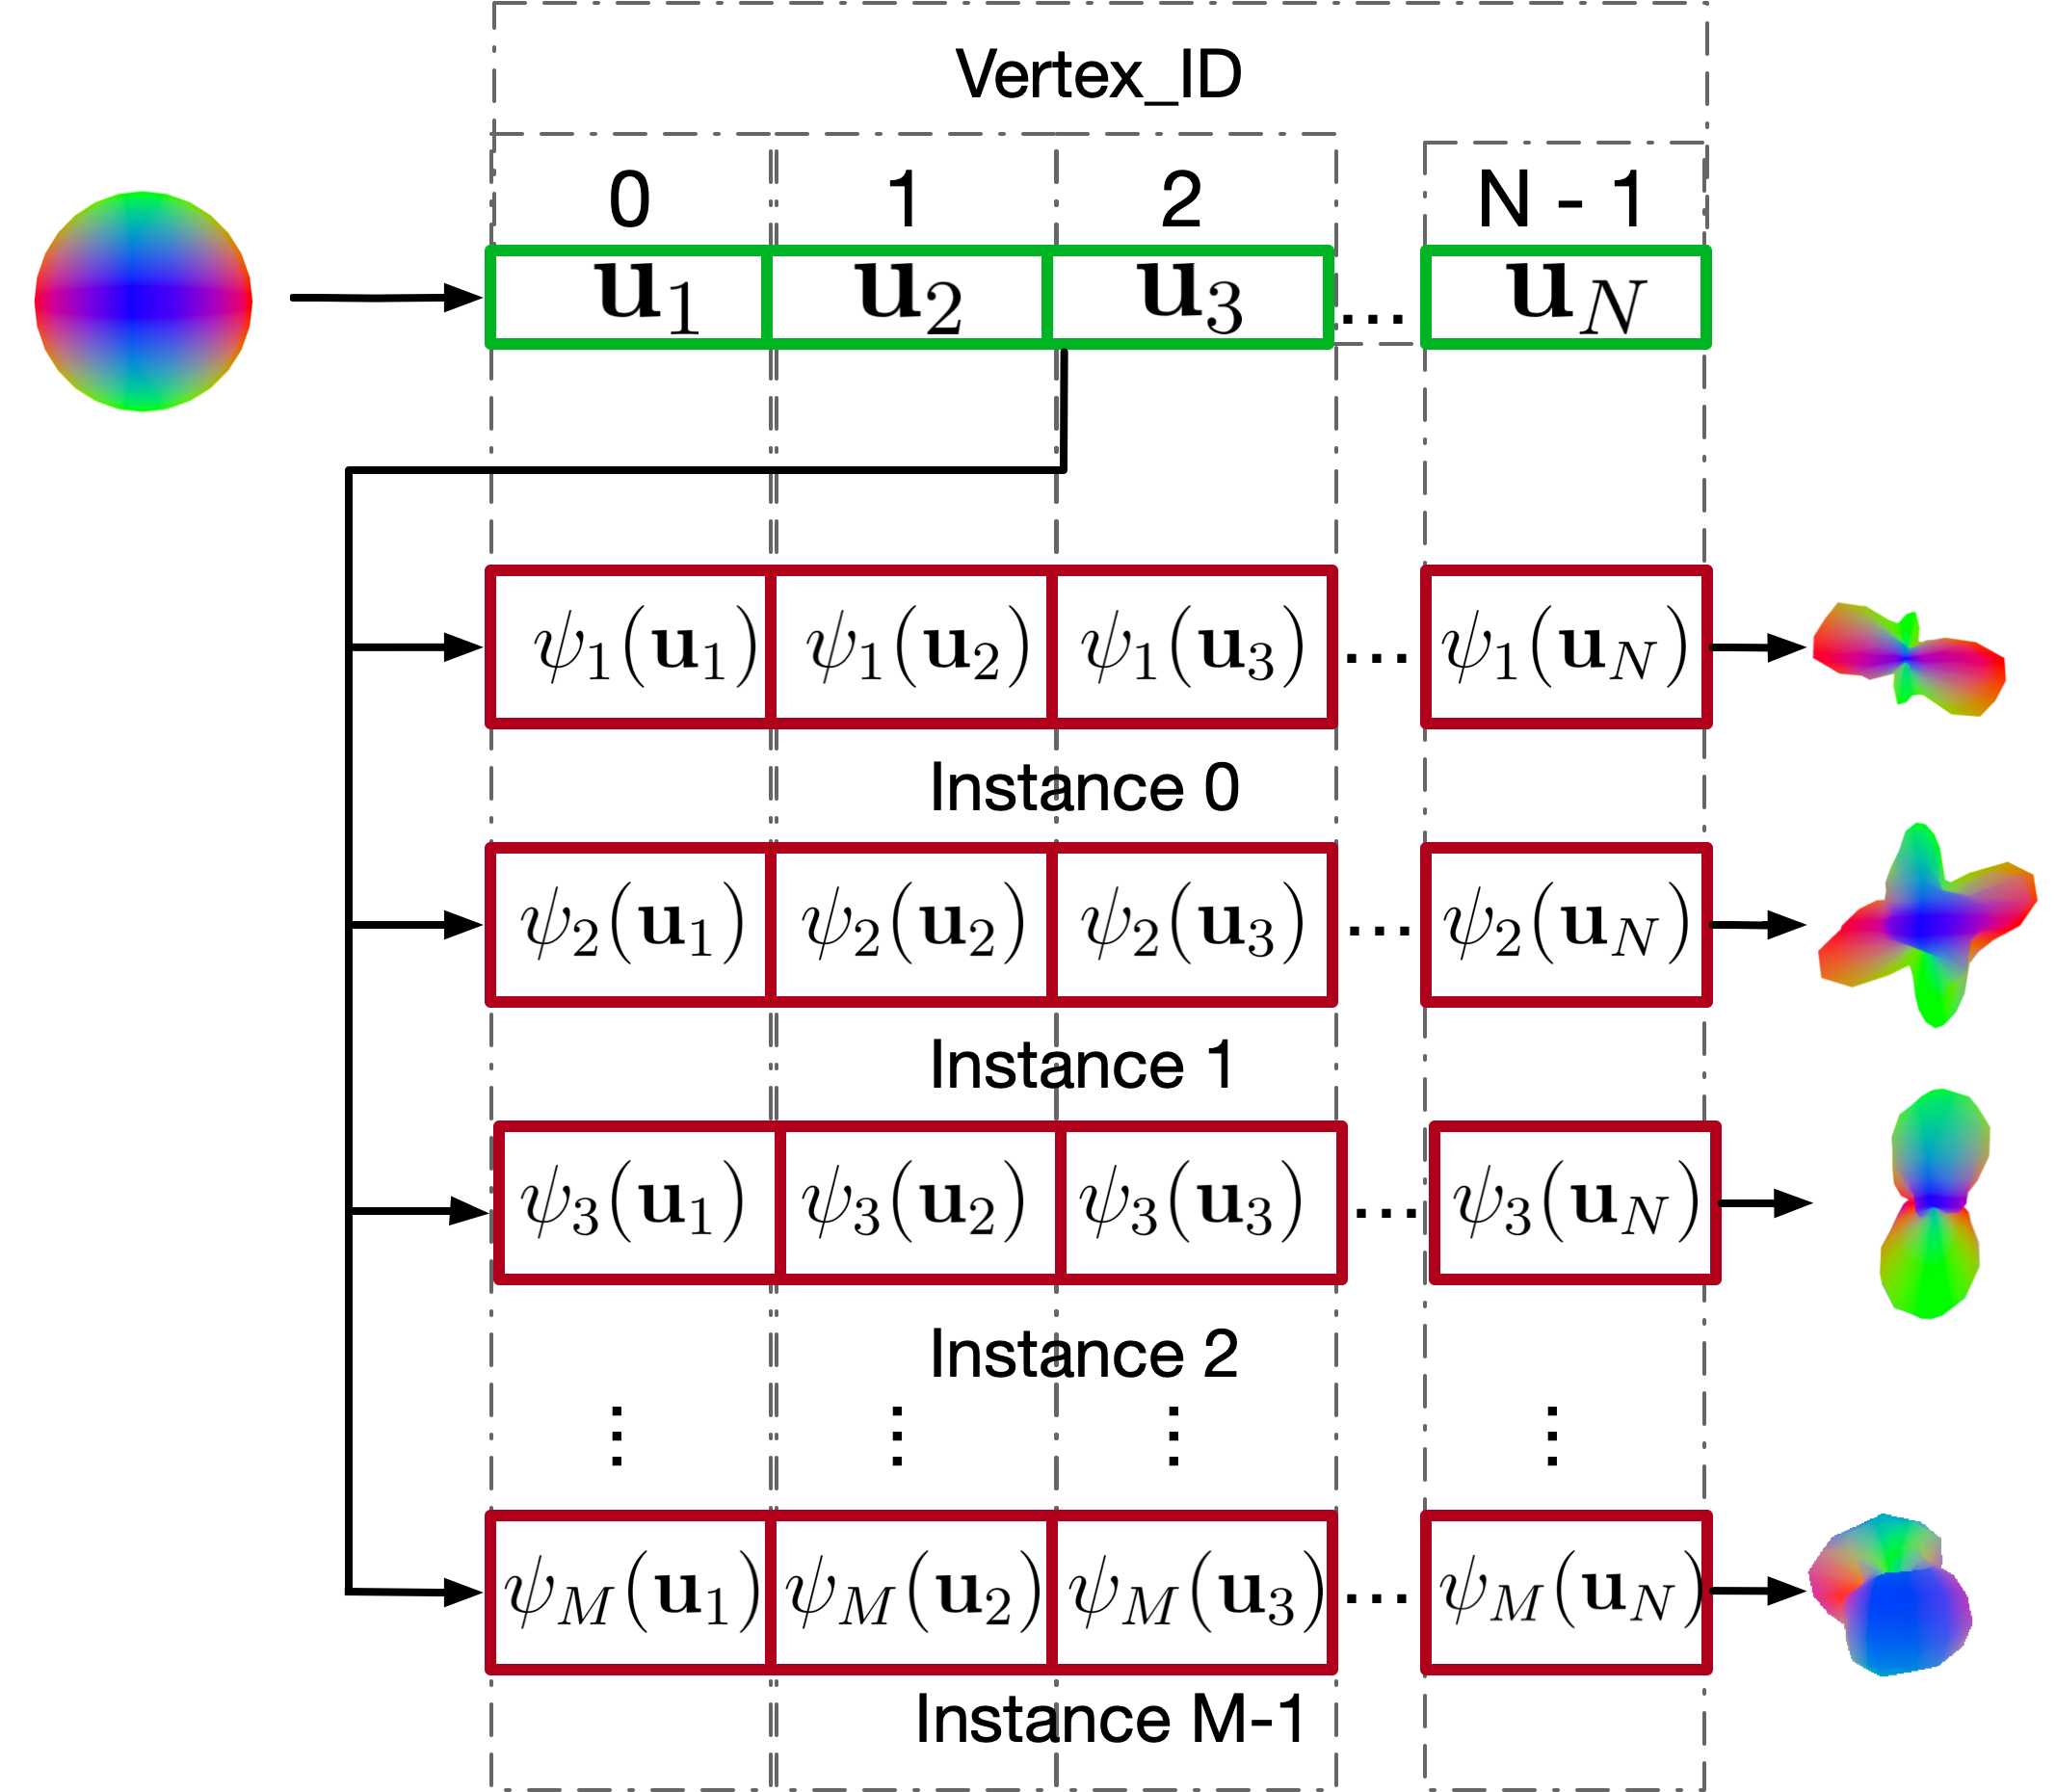
\includegraphics[width=1.0\linewidth, angle=0]{figs/rendering_scheme/GPU2Glyph.png}
    \caption{Illustration of the data organization in the GPU of the profile matrix (red) sent as 2D-Texture. The vertices of the spherical mesh are in green. At each instance, the customization of the glyph occurs through the multiplication of the mesh vertex with its respective value, recovered in the vertex shader through its vertex index for the P glyphs to be rendered.}
    \label{fig::GPU2glyph}
\end{figure}

\section{Results}

\subsection{Performance}


\section{Conclusions}







%\section{Page size}
%Permission to make digital or hard copies of all or part of this work for personal or classroom use is granted without fee provided that copies are not made or distributed for profit or commercial advantage and that copies bear this notice and the full citation on the first page. To copy otherwise, or republish, to post on servers or to redistribute to lists, requires prior specific permission and/or a fee. 

%All material on all pages should fit within a rectangle of 16 x 23.7 cm (6.3"x 9.33"), centered on the page horizontally, beginning 2.5 cm (1") from the top of the page and ending with 3,5 cm (1.4") from the bottom.  The right and left margins should be 2.5 cm (1"). The text should be in two 7.6 cm (3") columns with a 0.8 cm (0.3") gutter. 

%\section{Typeset text}
%\subsection*{Normal or Body Text}
%Please use a 10-point Times Roman font, or other Roman font with serifs, as close as possible in appearance to Times Roman in which these guidelines have been set. The goal is to have a 10-point text, as you see here. Please use sans-serif or non-proportional fonts only for special purposes, such as distinguishing source code text. If Times Roman is not available, try the font named Computer Modern Roman. On a Macintosh, use the font named Times.  Right margins should be justified, not ragged.

%\subsection*{Title and Authors}
%The title (Helvetica 18-point bold), authors' names (Helvetica 10-point) and affiliations (Helvetica 10 point) run across the full width of the page -- one column wide. We also recommend e-mail address (Helvetica 10 point). See the top of this page for three addresses. If only one address is needed, center all address text. For two addresses, use two centered tabs, and so on. For more than three authors, you may have to improvise.\footnote{If necessary, you may place some address information in a footnote, or in a named section at the end of your paper, but margins must remain empty.} 

%\subsection*{First Page Copyright Notice}
%Please include 3.8 cm (1.5") text box with the text shown at the bottom of the left column of the first page with the copyright notice.

%\subsection*{Others Pages}
%Others pages start at the top of the page (margin 2.5 cm) and continue in double-column format.  The two columns on the last even page should be as close to equal length as possible. 

%{\bfseries Total length of a paper is max. 8 pages.}

%Footnotes should be Times New Roman 9-point, and justified to the full width of the column.

%Please, use the standard Journal of WSCG format for references -- that is, a numbered list at the end of the article, ordered alphabetically by first author, and referenced by a name in brackets \cite{con00a}. See the examples of citations at the end of this document. Within this template file, use the style named references for the text of your citation.

%The references are also in 9 pt., but that section (see Section \ref{references}) is ragged right. References should be published materials accessible to the public. Internal technical reports may be cited only if they are easily accessible (i.e. you can give the address to obtain the report within your citation) and may be obtained by any reader. Proprietary information may not be cited. Private communications should be acknowledged, not referenced, e.g. "[Adam, personal communication]").

%\subsection*{Page Numbering, Headers and Footers}
%Do not include headers, footers or page numbers in your submission. These will be added when the publications are assembled.

%\begin{figure}[htb]
%    \centering
%    \rule{6cm}{3cm}
%    \caption{Insert caption to place caption below figure.}
%    \label{fig:box}
%\end{figure}

%\begin{table}[htb]
%	\centering
%	\begin{tabular}{|l|l|l|l|}
%	\hline
%	Graphics & Top & In-between & Bottom \\
%	\hline
%	Tables & End & Last & First \\
%	\hline
%	Figures & Good & Similar & Very well \\
%	\hline
%	\end{tabular}
%	\caption{Table captions should be placed below the table}
%\end{table}

%\section{Figures/Captions}
%Place Tables/Figures/Images in text as close to the reference as possible (see Fig.\ref{fig:box}). It may extend across both columns to a maximum width of 16 cm (6.3"). Captions should be Times New Roman 10-points.  They should be numbered (e.g., "Table 1" or "Figure 2"), please note that the word for Table and Figure are spelled out. Figure's and Table's captions should be centered beneath the image, picture or a table.

%\section{Sections}
%The heading of a section should be in Times New Roman 12-point bold in all-capitals flush left with an additional 6-points of white space above the section head.  Sections and subsequent sub- sections should be numbered and flush left. For a section head and a subsection head together (such as Section 3 and Subsection 3.1), use no additional space above the subsection head.

%\subsection{Subsections}
%The heading of subsections should be in Times New Roman 12-point bold with only the initial letters capitalized. (Note: For subsections and subsubsections, a word like the or a is not capitalized unless it is the first word of the header.)

%\subsubsection{Subsubsections}
%The heading for subsubsections should be in Times New Roman 11-point italic with initial letters capitalized and 6-points of white space above the subsubsection head.

%\section{Acknowledgments}
%Our thanks to ACM SIGCHI and SIGGRAPH for allowing us to modify templates they had developed.

%-------------------------------------------------------------------------
% example of algorithm typesetting
% to allow this, uncomment line 
% \RequirePackage[noend]{myalgorithm}
% in the wscg.sty file
% and download that package from Gabriel Zachmann's page http://zach.in.tu-clausthal.de/latex/
%
%
%\begin{algorithm}
%\hrule
%  \centering
%\begin{algorithmic}
%    \STMT $d_{l,r} = f_B(P_1), f_B(P_n)$
%    \WHILE{ $|d_l| > \epsilon $ and $|d_r| > \epsilon $ and $l<r$}
%        \STMT $d_x = f_B(P_x)$
%        \IF{ $d_x < 0$ }
%            \STMT $l, r = x, r$
%        \ELSE
%            \STMT $l, r = l, x$
%        \ENDIF
%    \ENDWHILE
%\end{algorithmic}
%\hrule
%\caption{Example of some pseudo-code}
%\label{fg:code}
%\end{algorithm}


%-------------------------------------------------------------------------

\printbibliography
%\begin{thebibliography}{99}
%\label{references}
%\label{references}
%\bibitem[And01a]{and01a} Anderson, R.E. Social %impacts of computing: Codes of professional %ethics. Social Science, pp.453-469, 2001.
%\bibitem[Con00a]{con00a} Conger., S., and Loch, %K.D. (eds.). Ethics and computer use. Com.of ACM %38, No.12, 2000.
%\bibitem[Con00b]{con00b} Mackay, W.E. Ethics, lies %and videotape, in Conf.proc. CHI'00, Denver CO, %ACM Press, pp.138-145, 2000.
%\bibitem[Jou01a]{jou01a} Journal of WSCG \& WSCG %templates: http://wscg.zcu.cz/jwscg/template.doc %(MSWord)
%http://wscg.zcu.cz/jwscg/template.pdf (PDF)
%\end{thebibliography}
%{\bfseries
%Last page should be fully used by text, figures etc. Do not leave empty space, please. 
%Do not lock the PDF -- additional text and info will be inserted, i.e. ISSN/ISBN etc. 
%}
\end{document}